%---------- Inleiding ---------------------------------------------------------

\section{Introductie}%
\label{sec:introductie}
Det tijd van programmeurs die code over de muur smijten en systeem adminstrators die alles manueel moeten opzetten is gedaan.
In hedendaagse dev/ops projecten moeten programmeurs (devs) en systeem administrators (ops) nauwer met elkaar samenwerken om na elke sprint een werkende versie van het project te realiseren.
Vandaag word door cloud based development de lijn tussen programmeurs en systeem administrators alsmaar waziger. 
Met het opkomen van Cloud based development is het simpelweg niet haalbaar om telkens opnieuw uw infrastructuur manueel aan te maken, dit zorgt ervoor dat men is overgestapt naar infrastructure as code (IAC).
Systeem administrators gaan met IAC de infrastructuur coderen zodanig dat men on the fly instanties kan bijmaken/aanpassen.
Ik had recent de vraag gekregen na een bedrijf waarbij ik op bezoek was om eens te kijken hoe moeilijk het is om te verwisselen van IAC taal
omdat ze graag zouden wisselen van hun huidig IAC softwarepacket (Bicep) naar een meer veelzijdig IAC softwarepacket (zoals bv Terraform).  
Dit is wat ik graag zou willen onderzoeken in deze paper.
Is het voor een bedrijf rendabel om hun Bicep code om te zetten naar Terraform code?



%---------- Stand van zaken ---------------------------------------------------

\section{State-of-the-art}%
\label{sec:state-of-the-art}
\subsection{Basisbegrippen}%

Wat is een Domain-Specific Language?
\\
In tegenstelling tot een algemene programmeer taal zoals C of UML is een domain-specific language(DSL)
ontworpen om statements in een bepaald probleemruimte of domein uit te drukken.
Bekende DSL's zijn reguliere expressies en SQL. Elke DSL is veel beter dan een algemene taal voor het beschrijven van bewerkingen op tekststrings of een database, 
maar veel slechter voor het beschrijven van ideeën die buiten zijn eigen scope liggen.
\autocite{DSL2022}

\subsection{Introductie Bicep}%

Bicep is begonnen als een open source DSL om de declarative deploment ervaring in Azure makkelijker te maken.
Bicep geeft een transparante, abstracte laag bovenop ARM templates en maakt het lezen en schrijven van Infrastructure as code in Azure veel makkelijker.
Bicep is het best te vergelijken met een transpiler; wanneer een Bicep file gecompileerd word, zal het de resources die omschreven zijn in de file vertalen naar een ARM template.
Een van de doelen van Bicep is om de huidige omslachtigheid rond ARM templates weg te halen door een abstractie laag bovenop de bestaande infrastructuur te geven.
Door deze manier kunnen mensen die nog niet in aanraking zijn gekomen met Azure een frictieloze manier hebben om met een native taal resouces to deploying naar Azure gebruikmakend van IAC.
\autocite{Rend_n_2022}
\begin{figure}[h!]
    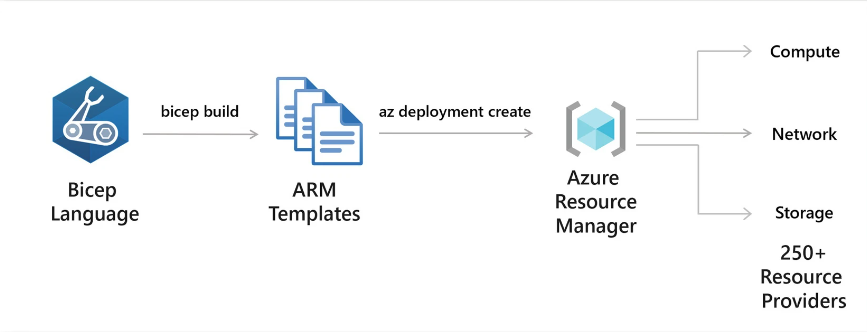
\includegraphics[width=.49\textwidth]{img/BicepSchema}
    \caption{Hoe Bicep Werkt met ARM}
    \label{fig:Bicep}
    \autocite{Rend_n_2022}
\end{figure}



\subsection{Wat is ARM?}%

ARM, ook gekend als Azure resource manager is de deployment and management service voor Azure. Heet geeft een management laag dat u in staat brengt om Azure resources in uw azure account te maken, updaten of deleten.
Nadat deze uitgevoerd zijn gebruikt ARM features zoals access controle, locks en tags om uw resources te beveiligen.
\autocite{ARM2022}
Om Infrastructure as code te kunnen implementeren voor Azure solutions gebruikt men ARM templates.
Het template is een JSON file da de configuratie van de infrastructuur vastlegt. ARM templates gebruiken declaratieve syntax, die ervoor zorgt dat men de staat waarin men wil deployen kan creëren  zonder dat je hiervoor een sequentie van programmeer commando's moet uitvoeren.
In het template moet enkel de resources die men wil deployen en zijn eigenschappen gespecificeerd worden.

Voordelen van ARM Templates:
\begin{itemize}
    \item Declaratieve Syntax: ARM templates zorgen ervoor dat je volledige Azure infrastructuren declaratief kan creëren
    Men kan bijvoorbeeld de netwerk infrastructuur, opslag systemen en elk anders resource dat men kan nodig hebben deploying, niet enkel virtuele machines
    \item Extensibility: Je kan via deployment scripts de volledige end-to-end omgeving  setup doen in 1 ARM template.
    \item Orchestration: Resouce Manager orchestrates de deployment van afhankelijke resources zodat ze in de correcte orde gecreëerd worden zodat je met 1 template en 1 commando alles kan opzetten.
    \item Preview changes: je kan doormiddel van een What-if operation verandering uittesten 
    zonder ze uit te voeren.
\end{itemize}
\autocite{ARMTemplates2022}


De Bicep taal is specifiek gemaakt door windows voor windows applicaties, dit zorgt natuurlijk voor een vlotte integratie met de Azure cloud hosting service van Windows.
Het grote nadeel van Bicep is deze taal enkel bruikbaar voor de Azure cloud enviroment dus het bedrijf zal genoodzaakt gebruik moeten maken van deze service.
Dit betekend conreet dat het bedrijf volledig afhankelijk is van Windows en zijn aanvullende services. Als het bedrijf wil overstappen naar een andere provider om zo meer flexibiliteit te geven aan haar klanten
zou het bedrijf haar volledige code base van Bicep moeten omvormen naar een andere taal. 

\subsection{Terraform}%

Terraform is een open source tool gemaakt door HashiCorp dat u toelaat om uw infrastructuur as code te definieren door middel van een simpele, declaratieve taal.
Deze taal kan men gebruiken om  uw infrastructuur te beheren en te deployen over verschillende public cloud providers (zoals: Amazon Web Services [AWS], Microsoft Azure, Google Cloud platform, DigitalOcean) 
en private cloud en vizualization platform (zoals OpenStack, VMware) gebruik makent van maar een paar simpele commando's.
Terraform is een zeer krachtige tool, het werkt met alle populaire cloud providers. Doordat terrafrom multi platform support aanbied geeft haar gebruikers de kans om dezelfde workflow te behouden irrelevant van de cloud provider,
dit maakt het bv mogelijk om een deel van uw infrastructuur te draaien op aws en daarnaast google cloud te gebruiken voor loadbalancing.    
\autocite{Oguejiofor2022}

Terrafrom gebuikt een eigen navitve language,HashiCorp configuration Language (HCL), een DSL die men kan gebruiken om infrastructuur configuratie te definiëren.
Terraform laat u infrastructuur en resources definiëren in een menselijk leesbare declaratieve configuratie bestanden, om zo de lifecycle van uw infrastructuur te beheren.
Voordelen van Terraform:
(hashi)
\begin{itemize}
    \item Terraform kan infrastructuur beheren op meerdere cloud platformen
    \item De menselijk leesbare aard van HCL maakt het makkelijk om snel infrastructuur code te schrijven
    \item Terraform state zorgt ervoor dat men de veranderingen in resources tussen alle deployments kan volgen.
    \item Terraform bied version control aan om zo een veilige collaboratie van uw infrastructuur te garanderen.
    
\end{itemize}
\autocite{Terraform2022}

% Voor literatuurverwijzingen zijn er twee belangrijke commando's:
% \autocite{KEY} => (Auteur, jaartal) Gebruik dit als de naam van de auteur
%   geen onderdeel is van de zin.
% \textcite{KEY} => Auteur (jaartal)  Gebruik dit als de auteursnaam wel een
%   functie heeft in de zin (bv. ``Uit onderzoek door Doll & Hill (1954) bleek
%   ...'')


%---------- Methodologie ------------------------------------------------------
\section{Methodologie}%
\label{sec:methodologie}

In een eerste fase van het onderzoek zullen we een gemaakte bicep file proberen omzetten naar een terraform file.
Dit houdt in dat een van de systeem beheerders een nieuwe file zal maken in Terraform die een analoge omgeving zal opzetten in een Azure cloud.
We gaan dit eerst kleinschalig uitvoeren  met 1 project.
Eens dat deze terraform file is aangemaakt kunnen we de gelijkenissen op vlak van functionaliteiten gaan bekijken en beide IAC talen een beoordeling geven.
Na dit praktisch onderzoek zullen we nog een theoretisch onderzoek ondernemen. 
We gaan kijken welke van de 2 IAC's het meeste features brengt (binnen azure) en welke van de 2 het meest veilig is.

%---------- Verwachte resultaten ----------------------------------------------
\section{Verwacht resultaat, conclusie}%
\label{sec:verwachte_resultaten}

Het feit dat terraform kan gedraaid worden op meerdere cloud providers kan een zeer goeie troef zijn die een bedrijf kan gebruiken om zijn services uit te breiden en de klant meer vrijheid te geven.
Maar als het aankomt op een infrastructur waar men enkel windows services gebruikt dan lijkt mij de logischeste keuze Bicep.
Het feit da Bicep tailor made is voor de microsoft omgeving geeft het een taktisch voordeel op terraform dus in Windows only enviroments lijkt mij de switch niet rendabel.
Als een bedrijf wil afstappen van zijn depencencie op microsoft of meer opties wil bieden aan de klant dan lijkt het mij een voor de hand liggende keuze om voor terraform te kiezen.
De keuze tussen Bicep of Terraform zal dus vooral afhangen van project tot project.

